\documentclass[french, a4paper, 10pt]{article}

\usepackage{babel}
\usepackage[T1]{fontenc}
\usepackage[utf8x]{inputenc}

\usepackage[top=2.5cm, bottom=2.5cm, left=2.5cm, right=2.5cm]{geometry}
\usepackage{float}
\usepackage{nicefrac}

\usepackage{chemist}
\usepackage{siunitx}
\usepackage{amsmath}
\usepackage{cases}

\usepackage[numbered,framed]{matlab-prettifier}

\DeclareSIUnit\jour{j}
\sisetup{per-mode=fraction, fraction-function=\nicefrac}
\newcommand{\dotc}[2]{\dot{#1}_{\text{\chemform{#2}}}}

\usepackage{etoolbox}
\newcommand{\ppath}[2][$\;\triangleright\;$]{%
	  \def\nextitem{\def\nextitem{#1}}% Separator
	    \renewcommand*{\do}[1]{\nextitem\textsf{##1}}% How to process each item
		  \docsvlist{#2}% Process list
	  }

\newcommand{\HRule}{\rule{\linewidth}{0.5mm}}

\fancyhf{} %clear all headers and footers fields
\fancyhead[R]{\thepage} %prints the page number on the right side of the header
\fancyhead[L]{Rapport de laboratoire CSTR}


\pagestyle{fancy}
\thispagestyle{empty}
\begin{titlepage}
\begin{center}

\includegraphics[width=0.15\textwidth]{pictures/logo.JPG}~\\[1cm]

\textsc{\LARGE Université Catholique de Louvain}\\[1.5cm]

\textsc{\Large Projet 3}\\[0.5cm]

% Title
\HRule \\[0.4cm]
{ \huge \bfseries Rapport de laboratoire CSTR\\[0.4cm] }

\HRule \\[1.5cm]

% Author and supervisor
\begin{minipage}{0.4\textwidth}
\begin{flushleft} \large
\textbf{Groupe \textsc{11.64}} \\
\textsc{Asselberghs} Paul \\
\textsc{Bertin} Brice \\
\textsc{Couplet} Adrien \\
\textsc{Crepeulandt} Grégory \\
\textsc{Gatin} Anthony \\
\textsc{Gennart} Antoine \\
\textsc{Gillard} Juline \\
\textsc{Martin} Pierre


\end{flushleft}
\end{minipage}
\begin{minipage}{0.4\textwidth}
\begin{flushright} \large
%\emph{Tuteur:} \\
%David \textsc{Cordova}
\end{flushright}
\end{minipage}

\setcounter{tocdepth}{2}
\tableofcontents % table des matières, totalement automatique ;)

\vfill

% Bottom of the page
{\large \today}
\end{center}
\end{titlepage}
%-----------------------------------------------------------
% début du document numéroté
\clearpage
\pagenumbering{arabic}
\newpage
%-----------------------------------------------------------

\thispagestyle{empty}


\begin{document}
\hypertitle{Thématique 2 : Gestion de la production}{LFSAB1503 Projet 3}{12.64}{Paul/Asselberghs, Brice/Bertin, Adrien/Couplet, Grégory/Creupelandt, Anthony/Gatin, Antoine/Gennart, Juline/Gillard, Pierre/Martin}{}{}{\today}

\tableofcontents\newpage

\part{Introduction}
Ce document a pour but d'étudier les bilans de matière et d'énergie d'un procédé alternatif de production d'ammoniac. Nous avons calculé pour chaque unité du procédé les débits d'entrée et de sortie ainsi que l'énergie et les températures dans l'unité de reformage autotherme. À partir des calculs obtenus dans ce document, il nous sera possible de développer un outil de simulation permettant d'étudier l'influence de paramètres sur le fonctionnement du procédé. 
\begin{figure}[h]
	\centering
	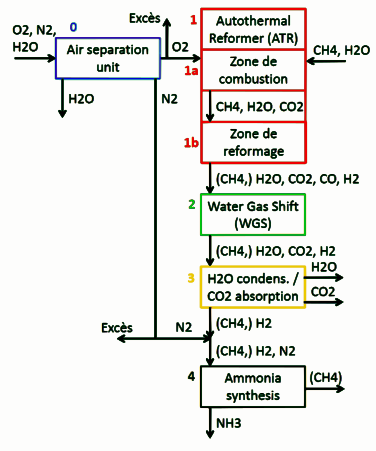
\includegraphics[width=0.5\textwidth]{pictures/procede.pdf}
	\caption{\label{fig:procede}Flow-sheet simplifié de la production d'ammoniac avec ATR}
\end{figure}

\section{Hypothèses}
Avant de commencer les calculs, il est necéssaire de faire quelques hypothèses afin de les simplifier : 
\begin{enumerate}
	\item La réaction de combustion de l'ATR (voir partie suivante, équation \ref{eq:combustion}) est considérée complète. Il n'en ressort que du \chemform{CO_2} et de l'\chemform{H_2O}. Normalement, dans le cas d'une combustion incomplète, un manque d'\chemform{O_2} aurait permit la formation de \chemform{CO} qui aurait interferé avec la suite du procédé.
	\item La réaction dans l'unité Water Gas Shift est considérée complète (équation \ref{eq:wgs}. Il est à noter que la même réaction survient plus tôt dans la zone de reformage mais de manière incomplète (équation \ref{eq:reformage2}). 
	\item Dans l'unité de condensation et d'absorption nous émettons l'hypothèse que nous retirons uniquement et complètement le \chemform{H_2O} et \chemform{CO_2} du procédé.
	\item En dehors des unités opérationelles, les réactifs ne réagissent pas entre eux.
	\item La réaction de synthèse de l'ammoniac (équation \ref{eq:synthese}) est considérée comme complète.
	\item Les quelconques pertes d'énergie entre les unités opérationelles sont négligeables. 
	\item Les paramètres initiaux qui nous sont donnés sont considérés comme exacts, sans marge d'erreur.
\end{enumerate}

\part{Bilan de matière}
Pour faciliter nos calculs nous considérons le symbole $\dot{n}$ comme étant le débit molaire avec comme unité le nombre de \si{\mol} produit par seconde.

Dans cette partie nous calculerons pour toutes les étapes du procédé les bilans de matière. À base de ceux-ci nous déterminerons les débits de production d'ammoniac, d'alimentation d'air, ainsi que tous les débits intermédiares entres les unités opérationnelles.

\section{Méthode de calcul des débits molaires}
Les débits molaires que nous utilisons dans nos calculs dépendent de l'unité dans laquelle ils sont calculés. Par exemple le $\dotc{n}{CH_4}$ de la zone de combustion n'est pas le même que celui de la zone de reformage. Au début de chaque unité nous reprenons les débits de l'unité précédente.
\subsection{ATR : zone de combustion}
Nous commencons par la zone de combustion où se produit la réaction chimique suivante :
	\begin{chemeqn}
		CH_4 + 2O_2 \longrightarrow CO_2 + 2H_2O
		\label{eq:combustion}
	\end{chemeqn}

\begin{table}[h]
	\centering\renewcommand{\arraystretch}{1.2}
	\begin{tabular}{l|ccccccc}
		& \chemform{CH_4} & + & \chemform{2O_2} & $\longrightarrow$ & \chemform{CO_2} & + & \chemform{2H_2O} \\\hline
		$\dot{n}_i$ & $\dotc{n}{CH_4}$ && $2\dotc{n}{O_2}$ && 0  && $\dotc{n}{H_2O}$  \\
		$\dot{n}_f$	& $\dotc{n}{CH_4}-\dotc{n}{O_2}$ && 0  && $\dotc{n}{O_2}$ && $\dotc{n}{H_2O}+2\dotc{n}{O_2}$ \\
	\end{tabular}
	\caption{\label{tab:combustion}Avancement de la combustion}
\end{table}

\subsection{ATR : Zone de reformage}
Deux équilibres chimiques ont lieu dans la zone de reformage. Ces deux réactions se déroulant simultanément, on ne peut les considérer séparement : 
\begin{chemeqn}CH_4+H_2O \rightleftharpoons 3H_2 + CO\label{eq:reformage1}\end{chemeqn}
\begin{chemeqn}CO + H_2O \rightleftharpoons H_2 + CO_2\label{eq:reformage2}\end{chemeqn}

\begin{table}[H]
	\centering\renewcommand{\arraystretch}{1.1}
	\begin{tabular}{l|ccccccc}
		& \chemform{CH_4} & + & \chemform{H_2O} & $\rightleftharpoons$ & \chemform{3H_2} & + & \chemform{CO} \\\hline 
		$\dot{n_0}$ & $\dotc{n}{CH_4}$ && $\dotc{n}{H_2O}$ && 0 && 0 \\
	   	$\dot{n_f}$ & $\dotc{n}{CH_4}-\xi$ && $\dotc{n}{H_2O}-\xi-\beta$ && $3\xi+\beta$ && $\xi-\beta$ \\	
	\end{tabular}
	\caption{\label{tab:reformage1}Avancement du premier équilibre chimique ($\xi$)}
\end{table}

\begin{table}[H]
	\centering\renewcommand{\arraystretch}{1.1}
	\begin{tabular}{l|ccccccc}
		& \chemform{CO} & + & \chemform{H_2O} & $\rightleftharpoons$ & \chemform{H_2} & + & \chemform{CO_2} \\\hline 
		$\dot{n_0}$ & 0 && $\dotc{n}{H_2O}$ && 0 && $\dotc{n}{CO_2}$ \\
	   	$\dot{n_f}$ & $\xi-\beta$ && $\dotc{n}{H_2O}-\xi-\beta$ && $3\xi+\beta$ && $\dotc{n}{CO_2}+\beta$ \\	
	\end{tabular}
	\caption{\label{tab:reformage2}Avancement du deuxième équilibre chimique ($\beta$)}
\end{table}

On déduit ensuite pour chaque équilibre l'expression de la constante d'équilibre :
\begin{align}
K_1 &= \frac{(\xi-\beta)(3\xi+\beta)^3}{(\dotc{n}{H_2O}-\xi-\beta)(\dotc{n}{CH_4}-\beta)}\cdot\frac{p_t^2}{(\dotc{n}{CH_4}+\dotc{n}{H_2O}+\dotc{n}{CO_2}+2\xi)^2}\\
K_2 &= \frac{(\dotc{n}{CO_2}+\beta)(3\xi+\beta)}{(\xi-\beta)(\dotc{n}{H_2O}-\xi-\beta)}
\end{align}
À partir de formules connues et de la température dans l'ATR donnée en paramètre nous pouvons déterminer les valeurss de $K_1$ et $K_2$ : 
$$ \begin{cases}K_1 &= 10^{\left(\frac{-11650}{T}+13.076\right)} \\
				K_2 &= 10^{\left(\frac{1910}{T}-1.764\right)} \end{cases}$$
Nous avons alors un système de deux équations à deux inconnues ($\xi$ et $\beta$). Nous résolvons ce système à l'aide du logiciel Matlab\textsuperscript{\textregistered} avec la fonction suivante :
\lstinputlisting[style=Matlab-editor, basicstyle=\footnotesize\ttfamily, tabsize=4, caption=Code Matlab\textsuperscript{\textregistered} pour résoudre le système]{ressources/reformage.m}
Au final, nous obtenons à la sortie de la zone de reformage les débits suivants :
\begin{table}[H]
	\centering\renewcommand{\arraystretch}{1.1}
	\begin{tabular}{l|ccccc}
		& \chemform{CH_4} & \chemform{H_2O} & \chemform{CO_2} & \chemform{CO} & \chemform{H_2}\\\hline
		$\dot{n_0}$ & $\dotc{n}{CH_4}$ & $\dotc{n}{H_2O}$ & $\dotc{n}{CO_2}$ & 0 & 0 \\
		$\dot{n_f}$ & $\dotc{n}{CH_4}-\xi$ & $\dotc{n}{H_2O}-\xi-\beta$ & $\dotc{n}{CO_2}+\beta$ & $\xi-\beta$ & $3\xi+\beta$
	\end{tabular}
	\caption{\label{tab:reformagetotal}Débits molaires d'entrée et de sortie de la zone de reformage}
\end{table}

\subsection{Water Gas Shift (WGS)}
Dans la zone de reformage se déroule déjà une réaction Water Gas Shift. Cette réaction se déroule de manière incomplète mais dans cette unité opérationnelle nous la considérons comme complète : 
\begin{chemeqn}CO + H_2O \longrightarrow CO_2 + H_2\end{chemeqn}

\begin{table}[h]
	\centering\renewcommand{\arraystretch}{1.2}
	\begin{tabular}{l|ccccccc}
		& \chemform{CO} & + & \chemform{H_2O} & $\longrightarrow$ & \chemform{CO_2} & + & \chemform{H_2} \\\hline
		$\dot{n}_i$ & $\dotc{n}{CO}$ && $\dotc{n}{H_2O}$ && $\dotc{n}{CO_2}$  && $\dotc{n}{H_2}$  \\
		$\dot{n}_f$	& 0 && $\dotc{n}{H_2O}-\dotc{n}{CO}$ && $\dotc{n}{CO_2}+\dotc{n}{CO}$ && $\dotc{n}{H_2}+\dotc{n}{CO}$ \\
	\end{tabular}
	\caption{\label{tab:wgs}Avancement de la réaction Water Gas Shift}
\end{table}


\subsection{Condensation et absorption}
Durant cette étapes aucune réaction chimique n'a lieu. Cette étape permet de retirer tout l'\chemform{H_2O} et le \chemform{CO_2} pour la suite du procédé. On considère que cette étape s'effectue complètement et qu'il ne reste plus aucune trace d'\chemform{H_2O} ou de \chemform{CO_2}.

\subsection{Synthèse de l'ammoniac}
Durant la dernière étape du procédé, nous synthétisons de l'ammoniac à partir d'hydrogène et d'azote :
\begin{chemeqn} 3H_2 + N_2 \longrightarrow 2NH_3 \end{chemeqn}

\begin{table}[h]
	\centering\renewcommand{\arraystretch}{1.2}
	\begin{tabular}{l|ccccc}
		& \chemform{3H_2} & + & \chemform{N_2} & $\longrightarrow$ & \chemform{2NH_3}\\\hline
		$\dot{n}_i$ & $\dotc{n}{H_2}$ && $\dotc{n}{N_2}$ && 0 \\
		$\dot{n}_f$	& $\dotc{n}{H_2}-3\dotc{n}{N_2}$ && 0  && $2\dotc{n}{N_2}$\\
	\end{tabular}
	\caption{\label{tab:synthese}Avancement de la synthèse de l'ammoniac}
\end{table}

\subsection{Air séparation unit}
Maintenant que nous connaissons les quantités nécessaires de \chemform{N_2} ainsi que celles de \chemform{O_2} qui interviennent dans l'ATR, nous pouvons déterminer la quantité d'air entrant dans l'unité de séparation d'air. Dans cette unité rentre de l'air composé de \chemform{O_2}, \chemform{N_2} et \chemform{H_2O}. En pourcentage cela nous donne : 21\% de \chemform{N_2} et 79\% de \chemform{O_2}. L'eau contenue dans l'air est négligeable et ressort directement après
séparation.
Le débit d'air entrant ainsi que les excès seront calculés numériquement dans la section suivante.

\section{Calcul numérique des débits}
Nos paramètres ainsi que leurs valeurs pour le cas précis sont les suivants :
\begin{table}[h]
	\centering\renewcommand{\arraystretch}{1.1}
	\begin{tabular}{lccl}\hline
		Paramètre & Valeur & Unité & Description \\\hline
		$\dotc{m}{CH_4}$ & 800 & \si{\tonne\per\jour} & Débit massique d'alimentation de \chemform{CH_4} \\
		$\nicefrac{\text{\chemform{O_2}}}{\text{\chemform{CH_4}}}$ & 0.6 & - & Rapport $\nicefrac{\text{\chemform{O_2}}}{\text{\chemform{CH_4}}}$ à l'entrée de l'ATR \\
		$\nicefrac{\text{\chemform{H_2O}}}{\text{\chemform{CH_4}}}$& 1.5 & - & Rapport $\nicefrac{\text{\chemform{H_2O}}}{\text{\chemform{CH_4}}}$ à l'entrée de l'ATR \\
		$T_{\text{ATR}}$ & 1200 & \si{\kelvin} & Température de la zone reforming de l'ATR \\
		$p_{\text{ATR}}$ & 50   & \si{\bar} & Pression d'opération de l'ATR \\\hline
	\end{tabular}
	\caption{\label{tab:parametres}Paramètres influant le fonctionnement du procédé}
\end{table}
\subsection{ATR}
\subsubsection{Zone de combustion}
\begin{table}[h]
	\centering\renewcommand{\arraystretch}{1.2}
	\begin{tabular}{ll|ccccccc}
		&& \chemform{CH_4} & + & \chemform{2O_2} & $\longrightarrow$ & \chemform{CO_2} & + & \chemform{2H_2O} \\\hline
		$\dot{m}_i$ & $[\si{\tonne\per\jour}]$ & 800 && 960 && 0 && 1350 \\
		$\dot{m}_i$ & $[\si{\kilo\gram\per\second}]$ \\
		$\dot{n}_i$ & $[\si{\mega\mol\per\jour}]$ & 50 && 30 && 0  && 75  \\\hline	
		$\dot{m}_f$ & $[\si{\tonne\per\jour}]$ & 560 && 0 && 660 && 1890 \\
		$\dot{m}_f$ & $[\si{\kilo\gram\per\second}]$ \\
		$\dot{n}_f$ & $[\si{\mega\mol\per\jour}]$ & 35 && 0 && 15 && 105 \\
	\end{tabular}
	\caption{\label{tab:rcombustion}Résultat de la combustion}
\end{table}

\subsubsection{Zone de reformage}
Suite à la résolution des équations nous obtenons les valeurs suivantes pour $\xi$ et $\beta$ :
$$\begin{cases}\xi &= \SI{28.992}{\mega\mol\per\jour}\\ \beta &= \SI{1.025}{\mega\mol\per\jour}\end{cases}$$
\begin{table}[h]
	\centering\renewcommand{\arraystretch}{1.2}
	\begin{tabular}{ll|ccccccc}
		&& \chemform{CH_4} & + & \chemform{H_2O} & $\rightleftharpoons$ & \chemform{3H_2} & + & \chemform{CO} \\\hline
		$\dot{m}_i$ & $[\si{\tonne\per\jour}]$ &  &&  &&  &&  \\
		$\dot{m}_i$ & $[\si{\kilo\gram\per\second}]$ \\
		$\dot{n}_i$ & $[\si{\mega\mol\per\jour}]$ & 35 && 105 && 0  && 0  \\\hline	
		$\dot{m}_f$ & $[\si{\tonne\per\jour}]$ &  \\
		$\dot{m}_f$ & $[\si{\kilo\gram\per\second}]$ \\
		$\dot{n}_f$ & $[\si{\mega\mol\per\jour}]$ & 6.008 && 74.983 && 88.001 && 27.967 \\
	\end{tabular}
	\caption{\label{tab:rcombustion}Résultat de la combustion}
\end{table}
\begin{table}[h]
	\centering\renewcommand{\arraystretch}{1.2}
	\begin{tabular}{ll|ccccccc}
		&& \chemform{CO} & + & \chemform{H_2O} & $\rightleftharpoons$ & \chemform{H_2} & + & \chemform{CO_2} \\\hline
		$\dot{m}_i$ & $[\si{\tonne\per\jour}]$ &  &&  &&  &&  \\
		$\dot{m}_i$ & $[\si{\kilo\gram\per\second}]$ \\
		$\dot{n}_i$ & $[\si{\mega\mol\per\jour}]$ & 0 && 105 && 0  && 15  \\\hline	
		$\dot{m}_f$ & $[\si{\tonne\per\jour}]$ &  \\
		$\dot{m}_f$ & $[\si{\kilo\gram\per\second}]$ \\
		$\dot{n}_f$ & $[\si{\mega\mol\per\jour}]$ & 27.967 && 74.983 && 88.001 && 16.025 \\
	\end{tabular}
	\caption{\label{tab:rcombustion}Résultat de la combustion}
\end{table}
\subsection{Water Gas Shift (WGS)}
\begin{table}[H]
	\centering\renewcommand{\arraystretch}{1.2}
	\begin{tabular}{ll|ccccccc}
		&& \chemform{CO} & + & \chemform{H_2O} & $\longrightarrow$ & \chemform{CO_2} & + & \chemform{H_2} \\\hline
		$\dot{m}_i$ & $[\si{\tonne\per\jour}]$ & \\
		$\dot{m}_i$ & $[\si{\kilo\gram\per\second}]$ \\
		$\dot{n}_i$ & $[\si{\mega\mol\per\jour}]$ & 27.967 && 74.983 && 16.025  && 88.001  \\\hline	
		$\dot{m}_f$ & $[\si{\tonne\per\jour}]$ &  \\
		$\dot{m}_f$ & $[\si{\kilo\gram\per\second}]$ \\
		$\dot{n}_f$ & $[\si{\mega\mol\per\jour}]$ & 0 && 47.016 && 43.992 && 115.969\\
	\end{tabular}
	\caption{\label{tab:rcombustion}Résultat de la combustion}
\end{table}
\subsection{Condensation et absorption}
$$\begin{cases} \dotc{n}{H_2O} &= 47.016 \\ \dotc{n}{CO_2} &= 43.992 \end{cases}$$
\subsection{Synthèse de l'ammoniac}
\begin{table}[H]
	\centering\renewcommand{\arraystretch}{1.2}
	\begin{tabular}{ll|ccccc}
		&& \chemform{3H_2} & + & \chemform{N_2} & $\longrightarrow$ & \chemform{2NH_3} \\\hline
		$\dot{m}_i$ & $[\si{\tonne\per\jour}]$ & \\
		$\dot{m}_i$ & $[\si{\kilo\gram\per\second}]$ \\
		$\dot{n}_i$ & $[\si{\mega\mol\per\jour}]$ & 115.969 && 38.656 && 0 \\\hline	
		$\dot{m}_f$ & $[\si{\tonne\per\jour}]$ &  \\
		$\dot{m}_f$ & $[\si{\kilo\gram\per\second}]$ \\
		$\dot{n}_f$ & $[\si{\mega\mol\per\jour}]$ & 0 && 0 && 77.312\\
	\end{tabular}
	\caption{\label{tab:rcombustion}Résultat de la combustion}
\end{table}
\subsection{Calcul des excès}
Pour l'\chemform{O_2} nous remarquons que nous n'avons pas d'excès. Car tout l'\chemform{O_2} présent dans l'air réagit dans l'ATR. 
Par contre pour le \chemform{N_2} la quantité présente dans l'air est de \SI{112.857}{\mega\mol\per\jour} et nous n'en utilisons que \SI{38.656}{\mega\mol\per\jour}.
Nous avons donc un excès de \SI{74.201}{\mega\mol\per\jour}.
\newpage

\part{Bilan d'énergie dans l'ATR}

\section{Méthode}

%%% Ajouter tableau des propriétés physico-chimique

Afin de déterminer la température d'entrée, on calcule l'enthalpie totale dégagée dans l'ATR et avec la formule \ref{eq:enthalpie} on peut déterminer la température initiale connaissant la température finale. 
\begin{equation}
	\Delta H_\text{tot} = c_{p,g}\Delta T
	\label{eq:enthalpie}
\end{equation}

\section{Résultats}
\subsection{Calcul de la température d'entrée dans l'ATR}
\subsubsection*{Zone de combustion}
On calcule dans un premier temps la variation d'enthalpie totale pour le nombre de moles de \chemform{CH_4} qui réagit.
\begin{chemeqn}
	2O_2 + CH_4 \longrightarrow CO_2 + 2H_2O
\end{chemeqn}
$$\Delta H^0_\text{\chemform{CH_4}} = \SI{-803}{\kilo\joule\per\mol}$$
$$\Delta\dot{H} = \SI{-12.045e9}{\kilo\joule\per\jour}$$

\subsubsection*{Zone de reformage}
On calcule ensuite la variation d'enthalpie pour les deux réactions incomplètes.
\begin{chemeqn}
	CH_4 + H_2O \rightleftharpoons 3H_2 + CO
\end{chemeqn}
$$\Delta H^0_\text{SMR} = \SI{224.0}{\kilo\joule\per\mol}$$
$$\Delta\dot{H} = \SI{6.4942e9}{\kilo\jour\per\jour}$$

\begin{chemeqn}
	CO + H_2O \rightleftharpoons H_2 + CO_2
\end{chemeqn}
$$\Delta H^0_\text{WGS} = \SI{-37.3}{\kilo\joule\per\mol}$$
$$\Delta\dot{H} = \SI{-38.2325e6}{\kilo\jour\per\day}$$

\subsubsection*{Total}
On somme ensuite toutes les variations d'enthalpie et utilisons la formule \ref{eq:dH}. Ainsi nous trouvons la température d'entrée dans l'ATR. Pour le débit massique total nous faisons la somme de tous les débits massiques entrant dans l'ATR.
\begin{align*}
	\Delta\dot{H}_\text{tot} &= \sum\Delta\dot{H}\\
							 &= \SI{-5.589e9}{\kilo\joule\per\jour} = \SI{-5.589e12}{\joule\per\jour}
\end{align*}
\begin{align*}
T_i &= \frac{-\Delta\dot{H}_\text{tot}+c_{p,g}\dot{m}_\text{tot}T_f}{c_{p,g}\dot{m}_\text{tot}}\\
&= \SI{1918.8}{\kelvin}
\end{align*}

\subsection{Calcul de la température finale dans la zone de combustion}
Dans ce cas ci, nous utilisons la même méthode que pour la température d'entrée. Au lieu de sommer toutes les variations d'enthalpie, nous utilisons celle de la zone de combustion. Le débit massique total reste identique.
\begin{align*}
T_f &= \frac{\Delta\dot{H}_\text{\chemform{CH_4}}+c_{p,g}\dot{m}_\text{tot}T_i}{c_{p,g}\dot{m}_\text{tot}}\\
&= \SI{369.6}{\kelvin}
\end{align*}

\end{document}



